\chapter{Design}
Using the data gathered in the previous chapter, we design a product that can solve the requirements, listed at section \ref{Requirements}. In this chapter we split the product into modular components that contain its functionality and use this to design the program architecture. Afterwards, we define interfaces to be used for implementing the software of the product. Besides the software, we also decide upon the physical design of the car, including which sensors we will use. Lastly, we will plan how we are going to test whether the individual components of the car conform to the requirements or not.

\section{Components}

To start, we split the project into a number of smaller modular components, that, when put together, make up a product that solves the requirements. The purpose of this is to gain an overview over the pieces of functionality required for the product, and the dependencies between these. Each component will be regarded as a wholly modular piece of the product, and will be tested separately from the rest. 

%Each component deals with only its own concerns

See figure \ref{fig:components} for the component diagram showing a separation of concerns into product components and their dependencies. On each component we've written the main functions that the component allows, abstracting away all low-level details. The arrows signify dependencies, e.g. that the manoeuvre-component requires the functions of the driving-component in order to work. 

\begin{figure}[ht]
    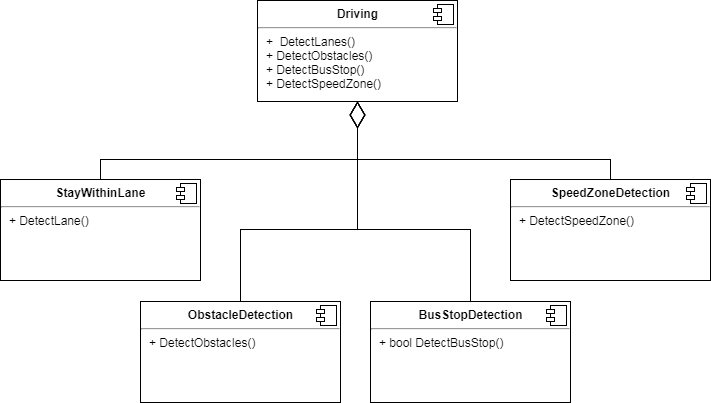
\includegraphics[width=\textwidth]{Images/Design/componentDiagram.png}
    \caption{Major components of functionality in the product; each component deals only with its own concerns}
    \label{fig:components}
\end{figure}
%Jeg er ikke overbevist om at ovenstående diagram er vildt vigtigt når vi nu alligevel har det nedenstående, dog giver det fint mening indtil videre

Note that the components refer not only to software, but also the physical design of the car. For instance, after we implement the driving component in software, we require a functioning LEGO-bus to test the software on. Only after this is done can we conclude whether the component works properly. Reason being that although the software logic might work as intended, incorrect sensor measurements, track/lane inconsistencies and similar need to be taken into account during programming, because otherwise the product might not work as expected.

\section{Software Architecture}
Using the separated components as the baseline, we create a class diagram that is less abstract than the component separation, which we will use as our software architecture. Using this diagram, we will later create precise interfaces for all its classes. The dark blue boxes signify the physical sensors that the program will need to communicate with. To better describe the concerns of each class on the diagram, we've written an example of one function call that might occur between the objects on each edge. This part isn't intended 

----

Used to create a class diagram for our implementation of the software architecture.
This is still, however, a bit of a simplification, because we can't get direct access to the sensors and actuators. 
The specifics of how we gain access to the sensors, we delegate to the light blue coloured objects named "API".

This is the model, ie. the logics of the program, so we don't wish to directly deal with these sorts of implementation and low-level details.


Example of the kind of function calls they do????


Diagram over our planned implementation, showing both classes and interfaces
Add function calls to the arrows? Or rather functions to the classes themselves?
This is still not one-to-one with implementation. The API's don't communicate directly with their corresponding sensors, instead they all query the NXT block, which gives access to different functions dependant on which sensors are connected.
Mention external bluetooth-sender program

\begin{figure}[ht]
    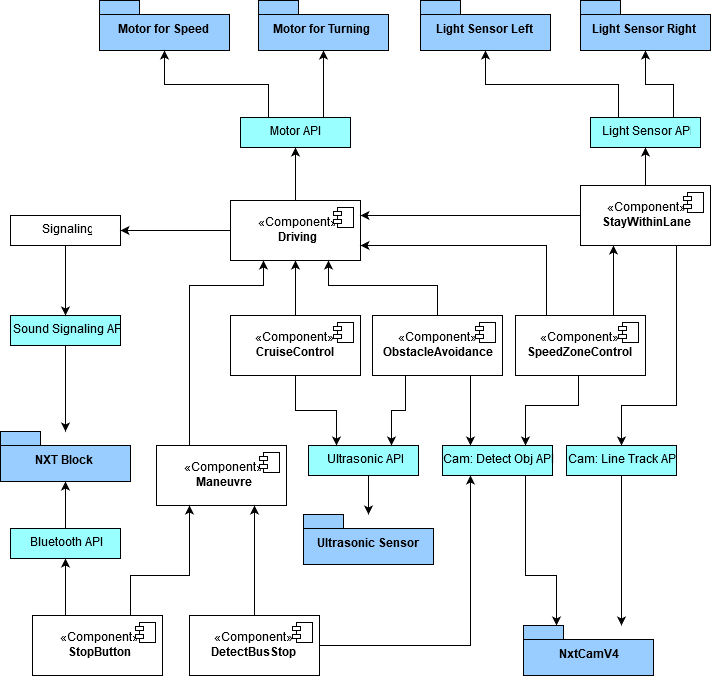
\includegraphics[width=\textwidth]{Images/Design/architectureClassDiagram.png}
    \caption{Diagram of the program architecture and how these communicate with each other}
    \label{give label}
\end{figure}

These classes will be used for implementing the program! It is still, however, kind of an abstraction.
In truth, the API's don't communicate directly with their corresponding sensors and actuators (and nxt block). 
Instead, they include libraries that facilitate this communication. 
The figure above shows the implementation of our model, ie. the software of the bus that we write ourselves.

Above this, there are many layers of abstraction in this project before one actually reaches the hardware level of the sensors. These are explained in the following section. 

\section{System Architecture}

Abstraction Layers, OS and nxtOSEK, lejOS?, ref to nxtOSEK section?

ABSTRACTION LAYER DIAGRAM
The frame "Components" in the figure are the components planned in the Software Architecture section. 

The diagram showing layers of abstraction in our design, including our NXTosek operating system

inclue ecrobot\_interface.h in source code
Write about the OSEK standard
And thereby also OIL
\begin{figure}[H]
    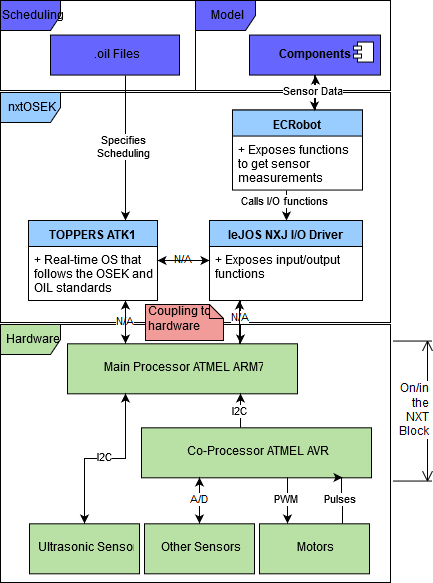
\includegraphics[width=\textwidth]{Images/Design/abstractionLayerDiagram.png}
    \caption{???}
\end{figure}

Add bluetooth maybe? Probably not, because it's a stub and therefore implementation-specific, not useful for the architecture


The attached ArchitectureClassDiagram describes what we intend for our model implementation. The idea is that we use this diagram directly for our program architecture, so that each object on the diagram becomes a class in the implementation. The light blue coloured API-object are classes that we will create ourselves. The intent with these is that they expose the useful functions that each sensor/actuator has, and also are the place where we calibrate our sensors (so, for instance, we filter out any incorrect measurements).

The attached AbstractionLayerDiagram describes our overall product architecture and abstractions, going from high-level programming to hardware specifics. Our model (eg. everything from the previous diagram) is contained inside the dark blue "Components"-box (purely the software, however). The note "coupling to hardware" exists because those are implementation details in nxtOSEK, which we don't really know about.


%\chapter{Design}
\section{Design of the track} \todo{This section needs to be checked for correctness.}

In order to fulfil the requirements of the project a track for the bus will have to be made, but before we can create the track it will first have to be designed.

The track should have two lanes, to mimic the pre-existing infrastructure with bidirectional roads. The track should furthermore have bus stops that the vehicle can drive into, such that passengers can get on/off the bus.
Furthermore the track should be designed to the scale of the bus, such that the turning rate of a corner should fit the maximum turning radius of the bus, and the width of the road should be designed after real danish roads based on the laws given by the danish road directorate \ref{} \todo{[MANLGER KILDE]}. Therefore the track needs be designed such that the bus has the needed space to turn around the corners without needing to reverse.

To help the sensors detect when to switch to a bus stop lane, the track should have special formed/coloured objects placed next to the bus stops, which the sensor(s) can recognise. Furthermore if any people are standing at the bus stop to get onto the bus, they should be placed close to the bus stop sign.

To draw the track that the bus will drive on, black tape should be used such that the sensors that perform line tracking can more easily detect and stay within the lines. Black has been chosen over white, even though white is normally used to draw track lines. But since white can be hard to detect because of light reflection the tracks will use black lines, this is to focus on a more complete bus implementation rather than focusing on tracking the lanes themselves.
\input{Documents/3Design/Design/Design_of_car}